\documentclass[10pt]{beamer}
\usetheme{Antibes}

\usepackage{graphicx}
\graphicspath{{../figures/}}


\title{Gendered Pronoun Resolution}
\author[Dhruv, Prateek]{ Dhruv Patel (14528) \and Prateek Sachan (15754)}
\institute[CSA, IISc.]{Computer Science and Automation, Indian Institute of Science}
\begin{document}
\begin{frame}
  \maketitle
\end{frame}

\section{Problem Introduction}
\begin{frame}{Problem}
  \begin{itemize}
  \item<+-> We are given a sentence or sentences, two candidate nouns within a sentence and a pronoun
  \item<+-> Task is to identify which of the two candidates referes to that pronoun
  \item<+-> Introduced as Kaggle competition by Google AI
  \end{itemize}

    \begin{block}<+->{Example}
      Impressed by her beauty, her warrior skills, and the fact that she was able to locate him, she is promoted to a position similar to that later held by her half-sister, Talia. As a right hand associate, she accompanies him during his adventures. Ra's is so impressed with her abilities, he even allows Nyssa to use his Lazarus Pits. Like \textit{\textbf{her}} sister \textbf{Talia}, \textbf{\underline{Nyssa}} eventually becomes disenchanted with Ra's genocidal plans to ``cleanse the Earth'', and disassociates herself from her father sometime in the early 20th century.
    \end{block}

\end{frame}

\section{Datasets}
\begin{frame}{Datasets}
  \begin{block}<+->{GAP Webster et al. (2018)\cite{webster2018gap}}
    
  \end{block}

  \begin{block}<+->{Definite Pronoun Resoluiton, Rahman et al. (2012), \cite{rahman2012resolving}}
    
  \end{block}

\end{frame}

\subsection{Data Augmentation}
\begin{frame}{Augmentation}

  \begin{itemize}
  \item One day before the battle, the astronomer- eunuch \textbf{Pu Wenying} came to see \textbf{Bao Daoyi}, warning him that he noticed an unlucky omen in the skies and urging \textbf{Bao} not to go to war. \textbf{Bao Daoyi} is furious after hearing \textbf{Pu Wenying}'s words and he slices \textbf{Pu} into two with his sword in anger.
  
  \item One day before the battle, the astronomer- eunuch \textbf{Ben Kuchera} came to see \textbf{David Cassidy}, warning him that he noticed an unlucky omen in the skies and urging \textbf{David} not to go to war. \textbf{David Cassidy} is furious after hearing \textbf{Ben Kuchera}'s words and he slices \textbf{Ben} into two with his sword in anger.
  
  \item "One day before the battle, the astronomer- eunuch \textbf{Irv Robbins} came to see \textbf{Jonas Schmidt}, warning him that he noticed an unlucky omen in the skies and urging \textbf{Jonas} not to go to war. \textbf{Jonas Schmidt} is furious after hearing \textbf{Irv Robbins}'s words and he slices \textbf{Irv} into two with his sword in anger.
    
  \end{itemize}
\end{frame}

\begin{frame}
  \begin{figure}
    \centering
    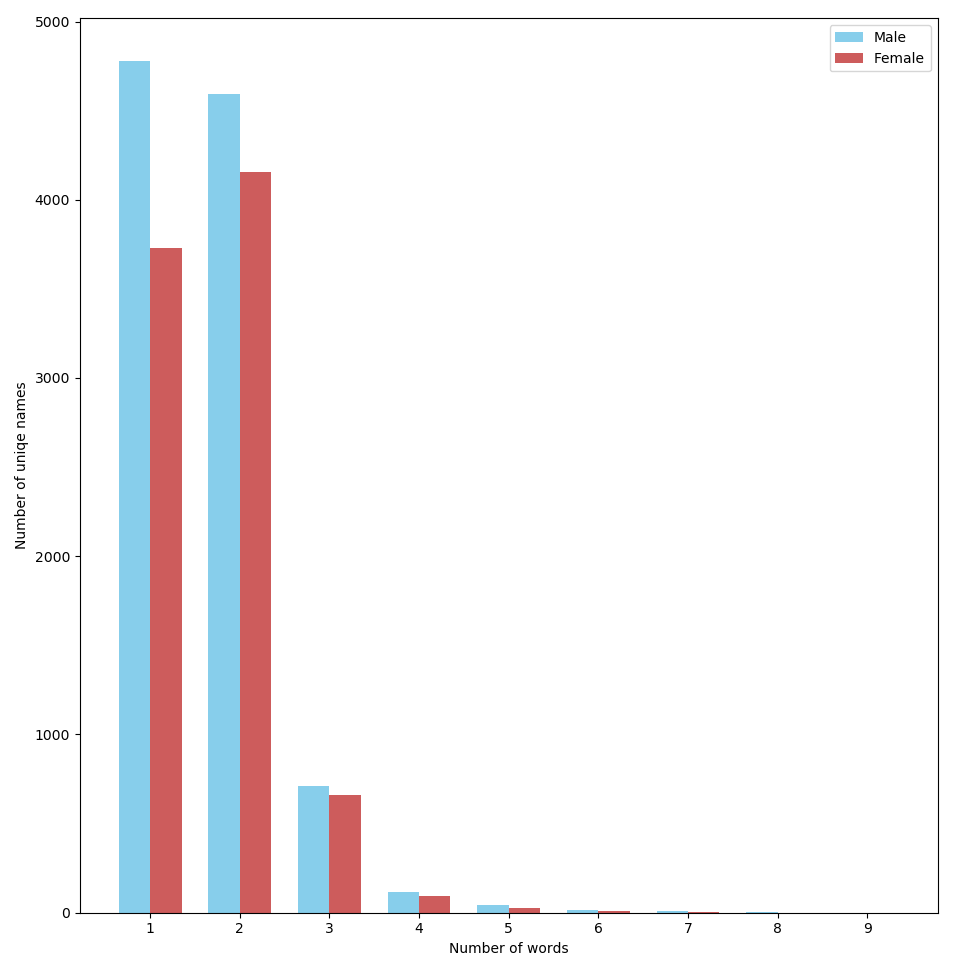
\includegraphics[width=.7\textwidth]{augment_dist.png}
    \caption{Distribution of names}
    \label{fig:dist_names}
  \end{figure}
\end{frame}

\section{}
\begin{frame}
  \frametitle{References}
  \bibliographystyle{ieeetr}
  \bibliography{presentation.bib}
\end{frame}

\end{document}